\chapter{Taking measurements}
This chapter is going to deal with finding an answer
to the question asked in section \ref{subsec:dev-skill-measurement}:
how to measure developer skill requirements from job advertisements.

%\section{Measuring job skill requirements}
%As stated in the abstract, technical interviews require more
%than the usual interview effort. In addition to personality
%tests that confirm that the candidate fits into the company
%culture, technical knowledge needs to be thoroughly checked.
%
%This is done in small programming exercises (either on-site or
%outsourced), examplary projects or by directly asking technically
%related questions during the interview itself.

\section{Job posting aspects}
By manually analyzing job offers from the Github Jobs
site\footnote{https://jobs.github.com}, it became clear that most
job offers consisted out of three parts:

\begin{itemize}
\item A description of the position environment
\item A detailed description of technical skill requirements
\item A "wishlist" about the employee character traits
\end{itemize}

Most startup job postings put the emphasis on candidate personality and
willingness to learn, as tasks and roles are not yet so clearly defined
at this stage of company life. For this reason mainly postings from larger, established companies were taken into account.
\newline

Inside this subset of openings, for example GitHub and Apple had very
specific, measureable technical requirements:
\newline

Apple wants candidates for a data engineer position to
\begin{itemize}
    \item have 3+ years experience with SQL
    \item have 3+ years experience with NoSQL
    \item know Hadoop
\end{itemize}

GitHub wants candidates to have experience
\begin{itemize}
    \item with web application backend, 3+ years
    \item with SQL
    \item with Ruby, JavaScript, ElasticSearch optionally
    \item with AWS or similar computing solutions optionally
\end{itemize}

Optional qualifications were always mentioned in conjunction with the
word "bonus". Presumably, candidates who receive bonuses are more
likely to get hired. Proficiency in a certain language is very well
verifiable by analyzing written source code, a technique that will
be looked at in detail in the next section.

\section{Determining developer skill}
Generally speaking, mastery of something is called a \textit{skill}.
Thus, a developer can call mastery of a technology a skill.
Measureable is only the code that the developer produces, which
is why this code will form the basis for analyzing the individual
developer skillset. This has the advantage that the analysis
can take historical data from the code repository into account
and be executed without the developers presence.

\section{Data source}
Analyzing closed source repositories is not an option, as there are lots
of privacy and security concerns. That is why the analysis will be
restricted to open source repositories.
\newline

GitHub is a popular open source community which enjoys high popularity
and hosts the source code repositories of a lot of high impact projects.
These include, but are of course not limited to,
Linux, git, docker, elasticsearch, flask and mongo\cite{rpfd:2014}.
More importantly, technical recruiters value profiles in such communities
greatly from applicants\cite{md:2013}, so there is an additional
incentive to this datasource. As repositories
often contain the combined works of multiple team members,
it is important that only individual contributions are measured.

\marginpar{96 out of 97 participants at HPI use GitHub.
608 HPI students and alumni were asked in this survey.}

Judging from the results of a small survey at the german Hasso-Plattner-Institute,
chances are that most passionate software developers own a GitHub account.\footnote{It should be
noted that HPI teaches IT-Systems Engineering \textit{exclusively}. The
survey reached 608 people.}
As such, GitHub provides a very good basis for data analysis.
It provides two types of data that are relevant for us: users and repositories.
\newline

A user provides the following relevant information:
\begin{itemize}
  \item A Name
  \item The number of followers and followings
  \item A biography with which the user describes himself
  \item A location
  \item Availability for hire
  \item E-Mail addresses which were used for committing
\end{itemize}
\vspace{2em}

\noindent A repository contains the development history of a project, which is subdivided into steps,
called \textit{commits}. In the following, we will be dealing with commits,
which carry the following attributes relevant for us (also depicted in Figure \ref{fig:commit}):

\begin{itemize}
    \item A \textit{date} when the commit was made
    \item An \textit{email} of whom made the commit
    \item A \textit{patch} of the changes made to the code
\end{itemize}

\begin{figure}
    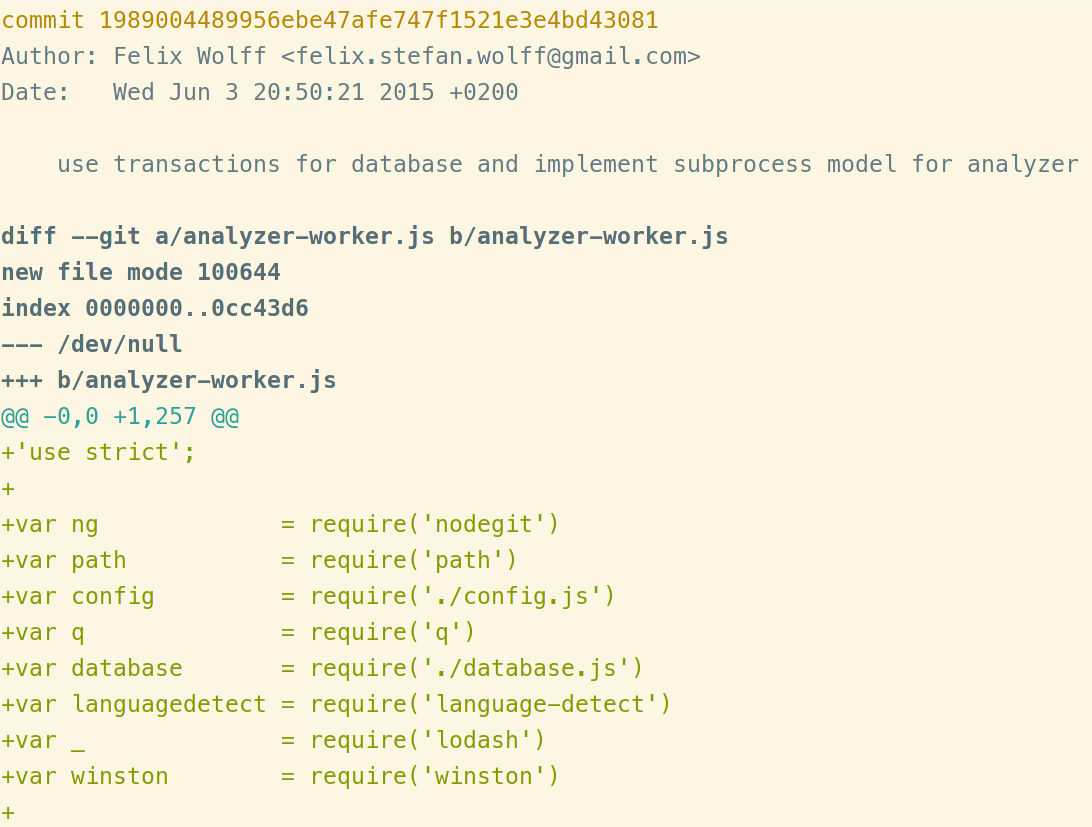
\includegraphics[width=30em]{gfx/commit.png}
    \caption{A sample commit displaying all of the relevant data: date, author with e-mail, diff}
    \label{fig:commit}
\end{figure}

\section{Constructing a metric}
%TODO
This section deals with constructing a metric for answering
the research question from \ref{subsec:dev-skill-measurement}.
At first, we will explore existing software sizing methods,
and how they relate to our intentional use.
The exploration was to no avail, as we will construct and defend
our own approach in the section after that.

\subsection{Existing software sizing methods}
Estimating software development effort is a task that
came up as early as 1981, when Barry W. Boehm invented the \textit{
Constructive Cost Model} (COCOMO)\footnote{\url{http://en.wikipedia.org/wiki/COCOMO}}.
It is a simple measure for estimating code cost
based on two main factors: developer count and development time.
\newline

It assumes that more developers will take \textit{less} time to produce the
same amount of code, measured in SLOCS\footnote{SLOCS is an abbreviation for
\textit{source lines of code}}.
This leads to the assumption that more developers produce more code.
The project itself does not grow, and thus more developers will finish it faster -
an epic wrong assumption of historical importance\cite{fb:1975}.
\newline

Research on other measurement methods clearly shows that measuring
function points\footnote{\url{http://en.wikipedia.org/wiki/Weighted_Micro_Function_Points}}\footnote{\url{http://www.projectcodemeter.com/cost_estimation/index.html}}
is state-of-the-art for measuring software size and complexity.\cite{linkedin:functionpointstandard}
A function point is the unit of measurement that expresses the amount of
business functionality a system provides to a user. This is a wholistic
measure, meaning that it analyzes the code as-is and does not take into
account individual contributions.

Clearly, measuring function points brings comparably better results
than counting SLOCs as it is programming language-agnostic and measures
the value of user-relevant program features, which makes it more
business-relevant. As a side note, counting SLOCs remains present in many
companies as processes have been formed around it. Some companies even resorted
to paying bonuses for higher line counts\cite{am:2009}.
\newline

Measuring wholistic development effort that has gone into a project as a
whole\footnote{\url{http://www.locmetrics.com/alternatives.html}}
is not the approach we need, because it does not take historical data from
version control systems into account and makes no distinction between
individual contributions.

\section{A custom metric}
The analyzed job offers ask for a minimum experience level with a certain technology.
Common code metrics however focus on code quality, and less on individual developer
productivity. All developer-focused metrics are seen with contempt
by both developers and managers \footnote{citation needed!!!!}
\newline

That is why we decided to construct a new metric which focuses on delivering a
satisfying answer to the first research question from \ref{subsec:dev-skill-measurement}.
Most large-scale projects make use of more than one programming language
or technology\footnote{see e.g. the \href{http://projects.apache.org/indexes/language.html}{Apache Software Foundation Programming Language Index}}, which is why language-sensitivity
needs to be part of our metric.

\subsection{A naive approach}
The data that was available to us consisted strictly out of commits and
code statistics. Two assumptions that came to our mindes were the following:

\begin{itemize}
 \item The more experienced a developer, the more code he has seen and written.
       This experience maps to a timespan worth working with this technology.
 \item Every human being is different, and as such, developers might have different learning paces.
       To attribute these, it makes sense to have experience as an abstract measure.
       This allows the metric to rank fast learners and slow learners on the same level,
       where the slow learner simply had more time.
\end{itemize}

Sadly, the only measurement we were able to make is the number of lines written.
As stated in section XYZ, Measuring SLOC is widely regarded as a bad practice.
It simply cannot be determined whether the writing of a line X has taken
ten seconds or five hours. And again, the kind of language used plays a huge role.
After lots of time spent into this, we diverted to another approach

there are different measures for each language and drawbacks of the SLOC approach
should be highlighted

\subsection{Technical fit}
From the data that each commit sports it is possible to say when a developer
used a programming language for the first time in a project.
By aggregating the data over several repositories, it is possible to say when
he has used it for the first time in general on GitHub.
This resolution of experience is based on timestamps and not on SLOC,
which has the disadvantage of being not accessible for fast learners
but relieves us of the neccessity to define a mapping of SLOC to a timespan.
By using the first and last dates \textit{d1} and \textit{d2} for commits
with a certain language, the timespan of experience with it can easily be
calculated, like in formula \ref{eq:timespan}. The function \textit{
julianday} converts dates into the number of days since January 1, 4713 BC.
It is based on the proleptic Julian calendar.

\begin{equation}
timespan = julianday(d2) - julianday(d1)
\label{eq:timespan}
\end{equation}

This simple calculation alone bears the fallacy that people who use a
programming language rarely but every few years get attributed lots
of experience. This is solved by the introduction of a \textit{productivity parameter},
which is based off the number of commits one makes per day - as formula \ref{eq:productivity} shows.

\begin{equation}
productivity = \frac{numberOfCommits}{timespan}
\label{eq:productivity}
\end{equation}

There is a downside to this, however. It rewards people who commit
large files of source code they have not written. A good example might be
a commit that contains the \textit{node\_modules} library folder from a
node.js project. In a single commit, this developer will have been
attributed thousands of lines of JavaScript. Small commits are generally
preferred \cite{so:commitsize}
over very large commits as they provide a better level of granularity for
reverting\footnote{git revert} or cherry-picking\footnote{git cherry-pick}.
For this reason, they have become more or less of a standard in
free open source software projects, with 50\% percent of all commits
being reasonably small \cite{rsk:2014}.
With this in mind, it makes sense to introduce another factor into
the metric that gives credit to developers who make small commits:

\begin{equation}
averageCommitSize = \frac{sum(linesPerCommit)}{count(commits)}
\label {eq:avgcommitsize}
\end{equation}

Combining all three values, the developers best suited for a position
\textit{from the technical perspective} are the ones who
have the \textit{greatest timespans}, the \textit{highest productivity},
but the \textit{lowest averageCommitSize}.

\subsection{Cultural fit}
Technical competencies aside, nobody wants to work with someone who does
not "fit in". A technical fit does not guarantee such a cultural fit.
GitHub provides precious little data for gaining insight into the
personality of a user.
\newline

A small indicator about the poularity of someone might be the way
his profile is valued. On GitHub, users can follow each other and be
notified of the actions of their followings. The value of these counters
might be a hint of importance and social acceptance.
\newline

GitHub used to provide users with the possibility to write about themselves.
Their API still provides a way to read this short biography\footnote{\url{https://developer.github.com/v3/users/}}, which is unfortunately a
remnant of the removal. This data will be removed in a future version,
which was confirmed upon question (see figure \ref{fig:gapitweet}).

\begin{figure}
  \centering
  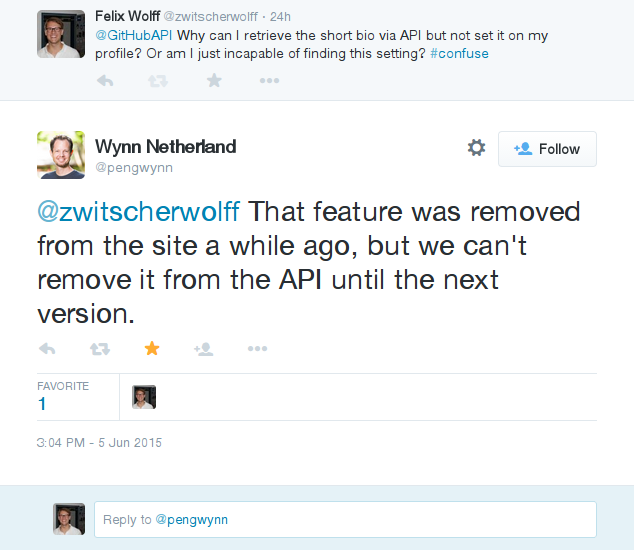
\includegraphics[width=25em]{gfx/githubapi_tweet.png}
  \caption{The tweet that confirmed that the \textit{bio} field is scheduled for removal}
  \label{fig:gapitweet}
\end{figure}

\section{Threats to validity}\label{sec:threatstovalidity}
For the metric to deliver meaningful results, the base data
needs to be sufficiently large and all e-mail addresses that were used for
making commits need to be registered with the GitHub profile.\\

Someone who used a open-source component at work, made a small bugfix,
and contributed it back into the project, but left his profile untouched
since then, will not have a very good standing because the data
for attaing one is simply missing. He may even be a very good developer
but any work not published to GitHub will not be considered.
